\documentclass{article}
\usepackage[utf8]{inputenc}
\usepackage{graphicx}
\graphicspath{{Imagens/}}


\title{Reprova Álgebra Linear}
\author{Gabriela Duarte Maciel e Augusto Rodrigo Camblor Santos }
\usepackage{geometry}
\geometry{a1paper,left=2cm,right=10mm,top=1cm,bottom=3cm}

\date{29 de outubro de 2022}

\begin{document}

\maketitle

\section{Exercício 1}\label{ex1}
Considere as bases do R−espaço vetorial R3, A = \{(4, 2, 0),(1, −1, 1),(5, 3, 3)\}  e
B = \{(1, −2, 1),(1, 5, 2),(1, 0, 1)\}. Exiba as matrizes de mudança de base MB→A e M_A→M_B. Escreva também os
vetores abaixo nas bases indicadas:
\\\textbf{• v = (0, 1, 2)A em B\\\\}
\\\textbf{• v = (1, 3, −1)B em A\\\\}
\section{Mudança M_B \rightarrow M_A_(_b_1_):}
\textbf{$x. a_1 + y. a_2 + z. a_3 = b_1 $\\\\}
x.(4, 2, 0) + y.(1, -1, 1) + z.( 5, 3, 3) = (1, -2, 1) \\\\

$
\xrightarrow{Inicio}
\begin{hbox}{

$\left[
\begin{tabular}{ccccc|c}
4 & 1 & 5 &  1\\
2 & -1 & 3 & -2\\
0 & 1 & 3 & 1\\
\end{tabular}
\right]

\textbf{l2 \rightarrow l2+l3}
\\\\
$\left[
\begin{tabular}{ccccc|c}
4 & 1 & 5 &  1\\
2 & 0 & 6 & -1\\
0 & 1 & 3 & 1\\
\end{tabular}
\right]
$}
\end{hbox}
\\\\\\\\\\
\xrightarrow{l1 \leftrightarrow l2}
\begin{hbox}{

$\left[
\begin{tabular}{ccccc|c}
2 & 0 & 6 & -1\\
4 & 1 & 5 &  1\\
0 & 1 & 3 & 1\\
\end{tabular}
\right]

$
$$\xrightarrow{l2\rightarrow l2-2.l1}
\\\\
$\left[
\begin{tabular}{ccccc|c}
2 & 0 & 6 & -1\\
0 & 1 & 7 &  3\\
0 & 1 & 3 & 1\\
\end{tabular}
\right]\\
$
\end{hbox}\\
\\\\\\\\\\
\xrightarrow{l3\rightarrow l3-l2}
\begin{hbox}{

$\left[
\begin{tabular}{ccccc|c}
2 & 0 & 6 & -1\\
0 & 1 & 7 &  3\\
0 & 0 & 10 & -2\\
\end{tabular}
\right]

$
$$\xrightarrow{l2\rightarrow 10.l2-7l3}
\\\\
$\left[
\begin{tabular}{ccccc|c}
2 & 0 & 6 & -1\\
0 & 10 & 0 &  16\\
0 & 0 & 10 & -2\\
\end{tabular}
\right]\\
$
\end{hbox}\\
\\\\\\\\\\
\xrightarrow{l1\rightarrow 10.l1-6.l3}
\begin{hbox}{

$\left[
\begin{tabular}{ccccc|c}
20 & 0 & 0 & 2\\
0 & 10 & 0 &  16\\
0 & 0 & 10 & -2\\
\end{tabular}
\right]

$
$$\xrightarrow{l1\rightarrow l1/20}
\\\\
$\left[
\begin{tabular}{ccccc|c}
1 & 0 & 0 & \(\frac{2}{20}\)\\\\
0 & 10 & 0 &  16\\\\
0 & 0 & 10 & -2\\
\end{tabular}
\right]\\
$
\end{hbox}\\
\\\\\\\\\\
\xrightarrow{l2\rightarrow l2/10}
\begin{hbox}{
$\left[
\begin{tabular}{ccccc|c}
1 & 0 & 0 & \(\frac{2}{20}\)\\\\
0 & 1 & 0 &  \(\frac{16}{10}\)\\\\
0 & 0 & 10 & -2\\
\end{tabular}
\right]

$
$$\xrightarrow{l3\rightarrow l3/10}
\\\\
$\left[
\begin{tabular}{ccccc|c}
1 & 0 & 0 & \(\frac{2}{20}\)\\\\
0 & 1 & 0 &  \(\frac{16}{10}\)\\\\
0 & 0 & 1 & \(\frac{-2}{10}\)\\
\end{tabular}
\right]\\
$
\end{hbox}\\
\\\\\\\\\\
\textbf{Coordenadas M_B\rightarrow M_A_(_b_1_): \\\\
a = \(\frac{1}{10}\); b = \(\frac{8}{5}\); c = \(\frac{-1}{5}\)\\\\}
\\\\\\\\\\

\section{Mudança de M_B \rightarrow M_A_(_b_2_):}\\\\
\textbf{$x. a_1 + y. a_2 + z. a_3 = b_2 $\\\\}
x.(4, 2, 0) + y.(1, -1, 1) + z.( 5, 3, 3) = (1, 5, 2) \\\\
\xrightarrow{Início}
\begin{hbox}{
$\left[
\begin{tabular}{ccccc|c}
4 & 1 & 5 &  1\\
2 & -1 & 3 & 5\\
0 & 1 & 3 & 2\\
\end{tabular}
\right]
$
$$\xrightarrow{l2\rightarrow l2+l3}
\\\\
$\left[
\begin{tabular}{ccccc|c}
4 & 1 & 5 &  1\\
2 & 0 & 6 & 7\\
0 & 1 & 3 & 2\\
\end{tabular}
\right]\\
$
\end{hbox}\\
\\\\\\
\xrightarrow{l1\leftrightarrow12}
\begin{hbox}{

$\left[
\begin{tabular}{ccccc|c}
2 & 0 & 6 & 7\\
4 & 1 & 5 &  1\\
0 & 1 & 3 & 2\\\
\end{tabular}
\right]

$
$$\xrightarrow{l2\rightarrow l2 - 2.l1}
\\\\
$\left[
\begin{tabular}{ccccc|c}
2 & 0 & 6 & 7\\
0 & 1 & -7 &  -13\\
0 & 1 & 3 & 2\\\
\end{tabular}
\right]\\\\\\\\
$
\end{hbox}\\
\\\\\\
\xrightarrow{l3\rightarrow 13-l2}
\begin{hbox}{

$\left[
\begin{tabular}{ccccc|c}
2 & 0 & 6 & 7\\
0 & 1 & -7 &  -13\\
0 & 0 & 10 & 15\\\
\end{tabular}
\right]

$
$$\xrightarrow{l3\rightarrow l3/10}
\\\\
$\left[
\begin{tabular}{ccccc|c}
2 & 0 & 6 & 7\\
0 & 1 & -7 &  -13\\
0 & 0 & 1 & \(\frac{15}{10}\)\\\
\end{tabular}
\right]\\
$
\end{hbox}\\
\\\\\\
\xrightarrow{l3\rightarrow \textbf{simplificando a fração: dividindo por 5}}
\begin{hbox}{

$\left[
\begin{tabular}{ccccc|c}
2 & 0 & 6 & 7\\
0 & 1 & -7 &  -13\\
0 & 0 & 1 & \(\frac{3}{2}\)\\
\end{tabular}
\right]

$
$$\xrightarrow{l2\rightarrow l2+7.l3}
\\\\
$\left[
\begin{tabular}{ccccc|c}
2 & 0 & 6 & 7\\
0 & 1 & 0 &  \(\frac{-5}{2}\)\\\\
0 & 0 & 1 & \(\frac{3}{2}\)\\
\end{tabular}
\right]\\
$
\end{hbox}\\
\\\\\\
\xrightarrow{l1\rightarrow l1 - 6.l3}
\begin{hbox}{

$\left[
\begin{tabular}{ccccc|c}
2 & 0 & 0 & -2\\
0 & 1 & 0 &  \(\frac{-5}{2}\)\\\\
0 & 0 & 1 & \(\frac{3}{2}\)\\
\end{tabular}
\right]

$
$$\xrightarrow{l1\rightarrow l1/2}
\\\\
$\left[
\begin{tabular}{ccccc|c}
1 & 0 & 0 & -1\\
0 & 1 & 0 &  \(\frac{-5}{2}\)\\\\
0 & 0 & 1 & \(\frac{3}{2}\)\\
\end{tabular}
\right]\\
\end{hbox}\\
\\\\\\
\textbf{Coordenadas M_B\rightarrow M_A_(_b_2_): \\\\
a = -1; b =  \(\frac{-5}{2}\); c = \(\frac{3}{2}\)\\\\}
\\\\

\section{Mudança de M_B \rightarrow M_A_(_b_3_):}\\\\
\textbf{$x. a_1 + y. a_2 + z. a_3 = b_3 $\\\\}
x.(4, 2, 0) + y.(1, -1, 1) + z.( 5, 3, 3) = (1, 0, 1) \\\\
\xrightarrow{Inicio}
\begin{hbox}{
$\left[
\begin{tabular}{ccccc|c}
4 & 1 & 5 &  1\\
2 & -1 & 3 & 0\\
0 & 1 & 3 & 1\\
\end{tabular}
\right]

$
$$\xrightarrow{l2\rightarrow l2+l3}
\\\\
$\left[
\begin{tabular}{ccccc|c}
4 & 1 & 5 &  1\\
2 & 0 & 6 & 1\\
0 & 1 & 3 & 1\\
\end{tabular}
\right]\\
\end{hbox}\\
\\\\\\

\xrightarrow{l1 \leftrightarrow l2}
\begin{hbox}{
$\left[
\begin{tabular}{ccccc|c}
2 & 0 & 6 & 1\\
4 & 1 & 5 &  -1\\
0 & 1 & 3 & 1\\
\end{tabular}
\right]

$
$$\xrightarrow{l2\rightarrow l2-2.l1}
\\\\
$\left[
\begin{tabular}{ccccc|c}
2 & 0 & 6 & 1\\
0 & 1 & -7 &  -1\\
0 & 1 & 3 & 1\\
\end{tabular}
\right]\\
\end{hbox}\\
\\\\\\

\xrightarrow{l3 \rightarrow l3-l2}
\begin{hbox}{
$\left[
\begin{tabular}{ccccc|c}
2 & 0 & 6 & 1\\
0 & 1 & -7 &  -1\\
0 & 0 & 10 & 2\\
\end{tabular}
\right]

$
$$\xrightarrow{l3 \rightarrow l3/10}
\\\\
$\left[
\begin{tabular}{ccccc|c}
2 & 0 & 6 & 1\\
0 & 1 & -7 &  -1\\
0 & 0 & 1 & \(\frac{2}{10}\)\\
\end{tabular}
\right]\\
\end{hbox}\\
\\\\\\

\xrightarrow{l1 \rightarrow l1 - 6.l3}
\begin{hbox}{
$\left[
\begin{tabular}{ccccc|c}
2 & 0 & 0 & \(\frac{-1}{5}\)\\\\
0 & 1 & -7 &  -1\\\\
0 & 0 & 1 & \(\frac{2}{10}\)\\
\end{tabular}
\right]

$
$$\xrightarrow{l2 \rightarrow l2 + 7.l3}
\\\\
$\left[
\begin{tabular}{ccccc|c}
2 & 0 & 0 & \(\frac{-1}{5}\)\\\\
0 & 1 & 0 &  \(\frac{2}{5}\)\\\\
0 & 0 & 1 & \(\frac{2}{10}\)\\
\end{tabular}
\right]\\
\end{hbox}\\
\\\\\\

\xrightarrow{l3 \rightarrow \textbf{simplificando a fração: dividindo por 2}}
\begin{hbox}{
$\left[
\begin{tabular}{ccccc|c}
2 & 0 & 0 & \(\frac{-1}{5}\)\\\\
0 & 1 & 0 &  \(\frac{2}{5}\)\\\\
0 & 0 & 1 & \(\frac{1}{5}\)\\
\end{tabular}
\right]

$
$$\xrightarrow{l1 \rightarrow l1/2}
\\\\
$\left[
\begin{tabular}{ccccc|c}
1 & 0 & 0 & \(\frac{-1}{10}\)\\\\
0 & 1 & 0 &  \(\frac{2}{5}\)\\\\
0 & 0 & 1 & \(\frac{1}{5}\)\\
\end{tabular}
\right]\\
\end{hbox}\\
\\\\\\
\textbf{Coordenadas M_B\rightarrow M_A_(_b_3_): \\\\
a = \(\frac{-1}{10}\); b = \(\frac{2}{5}\); c = \(\frac{1}{5}\)\\\\}
\\\\
\newpage
\section{Mudança de M_A \rightarrow M_B_(_A_1_)}
\textbf{$x. b_1 + y. b_2 + z. b_3 = a_1 $\\\\}
x.(1, -2, 1) + y.(1, 5, 2) + z.( 1, 0, 1) = (4, 2, 0) \\\\
\xrightarrow{Início}
\begin{hbox}{
$\left[
\begin{tabular}{ccccc|c}
1 & 1 & 1 & 4\\
-2 & 5 & 0 & 2 \\
1 & 2 & 1 & 0\\
\end{tabular}
\right]

$
$$\xrightarrow{l3 \rightarrow 5.l3 - 2.l2}
\\\\
$\left[
\begin{tabular}{ccccc|c}
1 & 1 & 1 & 4\\
-2 & 5 & 0 & 2 \\
9 & 0 & 5 & -4\\
\end{tabular}
\right]\\
\end{hbox}\\
\\\\\\

\xrightarrow{l1 \rightarrow 5.l1 - l2}
\begin{hbox}{
$\left[
\begin{tabular}{ccccc|c}
7 & 0 & 2 & 18\\
-2 & 5 & 0 & 2 \\
9 & 0 & 5 & -4\\
\end{tabular}
\right]

$
$$\xrightarrow{l1 \rightarrow l1 - l3}
\\\\
$\left[
\begin{tabular}{ccccc|c}
-2 & 0 & 0 & 22\\
-2 & 5 & 0 & 2 \\
9 & 0 & 5 & -4\\
\end{tabular}
\right]\\
\end{hbox}\\
\\\\\\

\xrightarrow{l2 \rightarrow l2 - l1}
\begin{hbox}{
$\left[
\begin{tabular}{ccccc|c}
-2 & 0 & 0 & 22\\
0 & 5 & 0 & -20 \\
9 & 0 & 5 & -4\\
\end{tabular}
\right]

$
$$\xrightarrow{l3 \rightarrow 2.l3 + 9.l1}
\\\\
$\left[
\begin{tabular}{ccccc|c}
-2 & 0 & 0 & 22\\
0 & 5 & 0 & -20 \\
0 & 0 & 10 & 190\\
\end{tabular}
\right]\\
\end{hbox}\\
\\\\\\

\xrightarrow{l1 \rightarrow l1/-2}
\begin{hbox}{
$\left[
\begin{tabular}{ccccc|c}
1 & 0 & 0 & -11\\
0 & 5 & 0 & -20 \\
0 & 0 & 10 & 190\\
\end{tabular}
\right]

$
$$\xrightarrow{l2 \rightarrow l2/5}
\\\\
$\left[
\begin{tabular}{ccccc|c}
1 & 0 & 0 & -11\\
0 & 1 & 0 & -4 \\
0 & 0 & 10 & 190\\
\end{tabular}
\right]\\
\end{hbox}\\
\\\\\\

\xrightarrow{l3 \rightarrow l3/10}
$\left[
\begin{tabular}{ccccc|c}
1 & 0 & 0 & -11\\
0 & 1 & 0 & -4 \\
0 & 0 & 1 & 19\\
\end{tabular}
\right]
$\\
\\\\\\
\textbf{Coordenadas M_A\rightarrow M_B_(_a_1_): a = -11; b = -4; c = 19\\\\}\\\\
\\\\



\section{Mudança de M_A \rightarrow M_B_(_A_2_)}
\textbf{$x. b_1 + y. b_2 + z. b_3 = a_2 $\\\\}
x.(1, -2, 1) + y.(1, 5, 2) + z.( 1, 0, 1) = (1, -1, 1) \\\\
\xrightarrow{Início}
\begin{hbox}{
$\left[
\begin{tabular}{ccccc|c}
1 & 1 & 1 & 1\\
-2 & 5 & 0 & -1 \\
1 & 2 & 1 & 1\\
\end{tabular}
\right]

$
$$\xrightarrow{l3 \rightarrow l3-l1}
\\\\
$\left[
\begin{tabular}{ccccc|c}
1 & 1 & 1 & 1\\
-2 & 5 & 0 & -1 \\
0 & 1 & 0 & 0\\
\end{tabular}
\right]\\
\end{hbox}\\
\\\\\\

\xrightarrow{l2 \leftrightarrow l3}
\begin{hbox}{
$\left[
\begin{tabular}{ccccc|c}
1 & 1 & 1 & 1\\
0 & 1 & 0 & 0\\
-2 & 5 & 0 & -1 \\
\end{tabular}
\right]

$
$$\xrightarrow{l1 \leftrightarrow l3}
\\\\
$\left[
\begin{tabular}{ccccc|c}
-2 & 5 & 0 & -1 \\
0 & 1 & 0 & 0\\
1 & 1 & 1 & 1\\
\end{tabular}
\right]\\
\end{hbox}\\
\\\\\\

\xrightarrow{l1 \rightarrow -1.l1}
\begin{hbox}{
$\left[
\begin{tabular}{ccccc|c}
2 & -5 & 0 & 1 \\
0 & 1 & 0 & 0\\
1 & 1 & 1 & 1\\
\end{tabular}
\right]

$
$$\xrightarrow{l1 \rightarrow l1 + 5.l2}
\\\\
$\left[
\begin{tabular}{ccccc|c}
2 & 0 & 0 & 1 \\
0 & 1 & 0 & 0\\
1 & 1 & 1 & 1\\
\end{tabular}
\right]\\
\end{hbox}\\
\\\\\\

\xrightarrow{l1 \rightarrow l1/2}
\begin{hbox}{
$\left[
\begin{tabular}{ccccc|c}
1 & 0 & 0 & \(\frac{1}{2}\) \\
0 & 1 & 0 & 0\\
1 & 1 & 1 & 1\\
\end{tabular}
\right]

$
$$\xrightarrow{l3 \rightarrow l3 - l2}
\\\\
$\left[
\begin{tabular}{ccccc|c}
1 & 0 & 0 & \(\frac{1}{2}\) \\
0 & 1 & 0 & 0\\
1 & 0 & 1 & 1\\
\end{tabular}
\right]\\
\end{hbox}\\
\\\\\\

\xrightarrow{l3 \rightarrow l3 - l1}
\begin{hbox}{
$\left[
\begin{tabular}{ccccc|c}
1 & 0 & 0 & \(\frac{1}{2}\) \\
0 & 1 & 0 & 0\\
0 & 0 & 1 & \(\frac{1}{2}\)\\
\end{tabular}
\right]
\end{hbox}\\
\\\\\\
\textbf{Coordenadas M_A\rightarrow M_B_(_a_2_): \\\\
a = \(\frac{1}{2}\); b = 0; c = \(\frac{1}{2}\)\\\\}
\\\\


\section{Mudança de M_A \rightarrow M_B_(_A_3_)}
\textbf{$x. b_1 + y. b_2 + z. b_3 = a_3 $\\\\}
x.(1, -2, 1) + y.(1, 5, 2) + z.( 1, 0, 1) = (5, 3, 3) \\\\
\xrightarrow{Início}
\begin{hbox}{
$\left[
\begin{tabular}{ccccc|c}
1 & 1 & 1 & 5\\
-2 & 5 & 0 & 3 \\
1 & 2 & 1 & 3\\
\end{tabular}
\right]

$
$$\xrightarrow{l3 \rightarrow 5.l3 - 2.l2}
\\\\
$\left[
\begin{tabular}{ccccc|c}
1 & 1 & 1 & 5\\
-2 & 5 & 0 & 3 \\
9 & 0 & 5 & 9\\
\end{tabular}
\right]\\
\end{hbox}\\
\\\\\\

\xrightarrow{l1 \rightarrow 5.l1 - l2}
\begin{hbox}{
$\left[
\begin{tabular}{ccccc|c}
7 & 0 & 5 & 22\\
-2 & 5 & 0 & 3 \\
9 & 0 & 5 & 9\\
\end{tabular}
\right]

$
$$\xrightarrow{l1 \rightarrow l1 - l3}
\\\\
$\left[
\begin{tabular}{ccccc|c}
-2 & 0 & 0 & 13\\
-2 & 5 & 0 & 3 \\
9 & 0 & 5 & 9\\
\end{tabular}
\right]\\
\end{hbox}\\
\\\\\\

\xrightarrow{l2 \rightarrow l2 - l1}
\begin{hbox}{
$\left[
\begin{tabular}{ccccc|c}
-2 & 0 & 0 & 13\\
0 & 5 & 0 & -10 \\
9 & 0 & 5 & 9\\
\end{tabular}
\right]

$
$$\xrightarrow{l3 \rightarrow 2.l3 + 9.l1}
\\\\
$\left[
\begin{tabular}{ccccc|c}
-2 & 0 & 0 & 13\\
0 & 5 & 0 & -10 \\
0 & 0 & 10 & 135\\
\end{tabular}
\right]\\
\end{hbox}\\
\\\\\\

\xrightarrow{l1 \rightarrow l1/-2}
\begin{hbox}{
$\left[
\begin{tabular}{ccccc|c}
1 & 0 & 0 & \(\frac{-13}{2}\)\\\\
0 & 5 & 0 & -10 \\
0 & 0 & 10 & 135\\
\end{tabular}
\right]

$
$$\xrightarrow{l2 \rightarrow l2/5}
\\\\
$\left[
\begin{tabular}{ccccc|c}
1 & 0 & 0 & \(\frac{-13}{2}\)\\\\
0 & 1 & 0 & -2 \\
0 & 0 & 10 & 135\\
\end{tabular}
\right]\\
\end{hbox}\\
\\\\\\

\xrightarrow{l3 \rightarrow l3/10}
\begin{hbox}{
$\left[
\begin{tabular}{ccccc|c}
1 & 0 & 0 & \(\frac{-13}{2}\)\\\\
0 & 1 & 0 & -2 \\\\
0 & 0 & 1 & \(\frac{135}{10}\)\\
\end{tabular}
\right]
\\\\
$$\xrightarrow{l3 \rightarrow \textbf{simplificando a fração: dividindo por 5}}
$\left[
\begin{tabular}{ccccc|c}
1 & 0 & 0 & \(\frac{-13}{2}\)\\\\
0 & 1 & 0 & -2 \\\\
0 & 0 & 1 & \(\frac{27}{2}\)\\
\end{tabular}
\right]\\
\end{hbox}\\
\\\\\\
\textbf{Coordenadas M_A\rightarrow M_B_(_a_3_): a = \(\frac{-13}{2}\); b = -2; c = \(\frac{27}{2}\)\\\\}\\\\
\\\\




\section{v = (1, 3, −1)B em A}

$
\mathbf{M_B \rightarrow _A:}
\begin{hbox}{

$\left[
\begin{array} {rrr}
\(\frac{1}{10}\) & -1 & \frac{-1}{10}\\\\
\(\frac{8}{5}\) & \(\frac{-5}{2}\) & \(\frac{2}{5})\\\\
\(\frac{-1}{5}\) & \frac{3}{2} & \frac{1}{5}\\\\
\end{array}
\right]
$
\textbf{.}
$\left[
\begin{array} {c}
1\\\\
3\\\\
-1\\\\
\end{array}
\right]
$
\\\rightarrow\\
$\left[
\begin{array} {rrr}
\(\frac{1}{10}\)*1 & -1*3 & \frac{-1}{10}*-1\\\\
\(\frac{8}{5}\)*1 & \(\frac{-5}{2}\)*3 & \(\frac{2}{5}\)*-1\\\\
\(\frac{-1}{5}\)*1 & \frac{3}{2}*3 & \frac{1}{5}*-1\\\\
\end{array}
\right]
$
\textbf{=}
$\left[
\begin{array} {c}
\frac{-14}{5}\\\\
\frac{-63}{10}\\\\
\frac{41}{10}\\\\
\end{array}
\right]
$}
\end{hbox}
\\\\\\


\section{v = (0, 1, 2)A em B}
\mathbf{M_A \rightarrow _B:}
\begin{hbox}{

$\left[
\begin{array} {rrr}
-11 & \frac{1}{2} & \frac{-13}{2}\\\\
4 & 0 & -2\\\\
19 & \frac{1}{2} & \frac{27}{2}\\\\
\end{array}
\right]
$
\textbf{.}
$\left[
\begin{array} {c}
0\\\\
1\\\\
2\\\\
\end{array}
\right]
$
\\\rightarrow\\
$\left[
\begin{array} {rrr}
-11*0 & \frac{1}{2}*1 & \frac{-13}{2}*2\\\\
4*0 & 0*1 & -2*2\\\\
19*0 & \frac{1}{2}*1 & \frac{27}{2}*2\\\\
\end{array}
\right]
$
\textbf{=}
$\left[
\begin{array} {c}
\frac{-25}{2}\\\\
-4\\\\
\frac{55}{2}\\\\
\end{array}
\right]
$}
\end{hbox}

\newpage

\section{Exercício 2}\label{ex2}
Considere o conjunto S = \{(1, 1, 1, 1, 1),(2, 0, −1, 1, 3),(3, 1, 0, 2, 4),(2, 2, 5, 8, −1),(0, 1, 0, 2, 3)\}.
\begin{itemize}
    \item S é LI ou LD?

\end{itemize}
\mathbf{S = }
\begin{hbox}{

$\left[
\begin{tabular}{ccccc|c}
1 & 2 & 3 & 2 & 0 & 0 \\
1 & 0 & 1 & 2 & 1 & 0 \\
1 & -1 & 0 & 5 & 0 & 0 \\
1 & 1 & 2 & 8 & 2 & 0 \\
1 & 3 & 4 & -1 & 3 & 0

\end{tabular}
\right]

\textbf{l2\leftarrow l2-1*l1}
\\\\
$\left[
\begin{tabular}{ccccc|c}
1 & 2 & 3 & 2 & 0 & 0 \\
0 & -2 & -2 & 0 & 1 & 0 \\
1 & -1 & 0 & 5 & 0 & 0 \\
1 & 1 & 2 & 8 & 2 & 0 \\
1 & 3 & 4 & -1 & 3 & 0


\end{tabular}
\right]
$}
\end{hbox}
\\\\\\\\\\
\xrightarrow{l3\rightarrow l3-1*l1}
\begin{hbox}{

$\left[
\begin{tabular}{ccccc|c}
1 & 2 & 3 & 2 & 0 & 0 \\
0 & -2 & -2 & 0 & 1 & 0 \\
0 & -3 & -3 & 3 & 0 & 0 \\
1 & 1 & 2 & 8 & 2 & 0 \\
1 & 3 & 4 & -1 & 3 & 0
\end{tabular}
\right]

$
$$\xrightarrow{l4\rightarrow l4-1*l1}
\\\\
$\left[
\begin{tabular}{ccccc|c}
1 & 2 & 3 & 2 & 0 & 0 \\
0 & -2 & -2 & 0 & 1 & 0 \\
0 & -3 & -3 & 3 & 0 & 0 \\
0 & -1 & -1 & 6 & 2 & 0 \\
1 & 3 & 4 & -1 & 3 & 0
\end{tabular}
\right]\\
$
\end{hbox}\\
\\\\\\\\\\
\xrightarrow{l5\rightarrow l5-1*l1}
\begin{hbox}{

$\left[
\begin{tabular}{ccccc|c}
1 & 2 & 3 & 2 & 0 & 0 \\
0 & -2 & -2 & 0 & 1 & 0 \\
0 & -3 & -3 & 3 & 0 & 0 \\
0 & -1 & -1 & 6 & 2 & 0 \\
0 & 1 & 1 & -3 & 3 & 0
\end{tabular}
\right]

$
$$\xrightarrow{l3\rightarrow l3-(3/2)*l2}
\\\\
$\left[
\begin{tabular}{ccccc|c}
1 & 2 & 3 & 2 & 0 & 0 \\
0 & -2 & -2 & 0 & 1 & 0 \\
0 & 0 & 0 & 3 & (-3/2) & 0 \\
0 & -1 & -1 & 6 & 2 & 0 \\
0 & 1 & 1 & -3 & 3 & 0
\end{tabular}
\right]\\
$
\end{hbox}\\
\\\\\\\\\\
\xrightarrow{l4\rightarrow l4-(1/2)*l2}
\begin{hbox}{

$\left[
\begin{tabular}{ccccc|c}
1 & 2 & 3 & 2 & 0 & 0 \\
0 & -2 & -2 & 0 & 1 & 0 \\
0 & 0 & 0 & 3 & (-3/2) & 0 \\
0 & 0 & 0 & 6 & (-3/2) & 0 \\
0 & 1 & 1 & -3 & 3 & 0
\end{tabular}
\right]

$
$$\xrightarrow{l5\rightarrow l5-(-1/2)*l2}
\\\\
$\left[
\begin{tabular}{ccccc|c}
1 & 2 & 3 & 2 & 0 & 0 \\
0 & -2 & -2 & 0 & 1 & 0 \\
0 & 0 & 0 & 3 & (-3/2) & 0 \\
0 & 0 & 0 & 6 & (3/2) & 0 \\
0 & 0 & 0 & -3 & (7/2) & 0
\end{tabular}
\right]\\
$
\end{hbox}\\
\\\\\\\\\\
\xrightarrow{l4\rightarrow l4-2*l3}
\begin{hbox}{

$\left[
\begin{tabular}{ccccc|c}
1 & 2 & 3 & 2 & 0 & 0 \\
0 & -2 & -2 & 0 & 1 & 0 \\
0 & 0 & 0 & 3 & (-3/2) & 0 \\
0 & 0 & 0 & 0 & (9/2) & 0 \\
0 & 0 & 0 & -3 & (7/2) & 0
\end{tabular}
\right]

$
$$\xrightarrow{l5\rightarrow l5-(-1)*l3}
\\\\
$\left[
\begin{tabular}{ccccc|c}
1 & 2 & 3 & 2 & 0 & 0 \\
0 & -2 & -2 & 0 & 1 & 0 \\
0 & 0 & 0 & 3 & (-3/2) & 0 \\
0 & 0 & 0 & 0 & (9/2) & 0 \\
0 & 0 & 0 & 0 & 2 & 0

\end{tabular}
\right]\\
$
\end{hbox}\\
\\\\\\\\\\
\xrightarrow{l5\rightarrow l5-(-4/9)*l4}
\begin{hbox}{

$\left[
\begin{tabular}{ccccc|c}
1 & 2 & 3 & 2 & 0 & 0 \\
0 & -2 & -2 & 0 & 1 & 0 \\
0 & 0 & 0 & 3 & (-3/2) & 0 \\
0 & 0 & 0 & 0 & (9/2) & 0 \\
0 & 0 & 0 & 0 & 0 & 0
\end{tabular}
\right]\\
$
\end{hbox}\\
\\\textit{R: Portanto, é LD}\\\\
\begin{itemize}
   \item Forma base do R-espaço vetorial R5?
   \\\textit{R:Como S é ld, ele não forma uma base de R^5}
\end{itemize}












































































    
\end{hbox}
\newpage
\section{Exercício 3}\label{ex3}
 Considere o conjunto W = \{(x, y, z, w, t, u) \mid  x, y, z, w, t, u \in R \land x + y + w + z + t + u = 0 \land y -  w - z = 0 \land w + t - x = 0\} \subseteq R^6. 


\item Mostre que conjunto W é um subespaço do R-espaço vetorial R^6 .

\\t – x = 0 

t = x 

y – w – z = 0 

y = w + z 

x + y + w + z + t + u = 0 \to  x + w + z + w + z + x + u = 0 

u = -x -y -w -z -t \to u = -2x -2w -2z 

W = \{(x, w + z, z, w, x, - x – w – z – w – z – x)\} \to

W = \{(x, w + z, z, w, x, - 2x – 2w – 2z)\mid x, z, w \in R\}\\

I) 0 \in W para x = 0 z = 0 w = 0 

(w, w, w, w, w, -w) \to (x, w + z, z, w, x, - 2x – 2w – 2z) 

= (0, 0, 0, 0, 0, -0) 

= 0 

Logo, 0 \in W\\ 

II) u, z \in W \to  u + z \in W, sendo:  

u = (u1, u2, u3, u4, u5, -u6) \to (x_1, w_1 + z_1, z_1, w_1, x_1, - 2x_1 – 2w_1 – 2z_1) 

z = (z1, z2, z3, z4, z5, -z6) \to (x_2, w_2 + z_2, z_2, w_2, x_2, - 2x_2 – 2w_2 – 2z_2)  

u + z = (x_1 + x_2, (w_1+z_1) + (w_2+z2) , z_1 + z_2, w_1 + w_2, x_1 + x_2, (-2x_1 -2w_1 - 2z_2) + (-2x_2 - 2w_2 - 2z_2)) 

u + z= (x_1 + x_2, w_1+z_1+w_2+z_2, z_1+z_2, w_1+w_2, x_1+x_2, -2x_1-2x_2,-2w_1-2w_2,-2z_1-2z_2) 

Logo, u + z \in W \\

III) a \in R, v \in W \to av \in W, sendo:  

v = (v1, v2, v3, v4, v5, -v6) \to (x, w + z, z, w, x, - 2x – 2w – 2z) 

av = a . (x_1, w_1+z_1, z_1, w_1, x_1, -2x_1-2w_1-2z_1) 

 av = (a. x_1, a . w_1+z_1, a . z_1, a . w_1, a . x_1, a. -2x_1-2w_1-2z_1)  

av = (ax_1, aw_1w_2, az_1, aw_1, ax_1, a-2x_1-2w_1-2z_1) 

Logo, av \in W. \\

Logo W é subespaço vetorial de R6.\\

\begin{itemize}
\\\item O conjunto W = \{(x, y, z) \mid  x, y, z \in R \land x - z = 1 \land  y + x = 0\} \end{itemize}
    
    \item é um subsespaço vetorial de R3? Esboce graficamente W.\\

x – z = 1 \to x = 1 + z

y + x = 0 \to y + 1 + z = 0 \to y = -1 – z. 

W = \{(1 + z, -1 - z, z)\} \\

I) 0 \in W, para z = 0 

(1 + z, - 1 – z, z) \to (1 + 0, - 1 – 0, 0) = (1, -1, 0).  

Logo 0 NÃO pertence a W para z = 0. Portanto, W NÃO é subespaço vetorial.\\ 

\begin{figure}[!h]
\centering
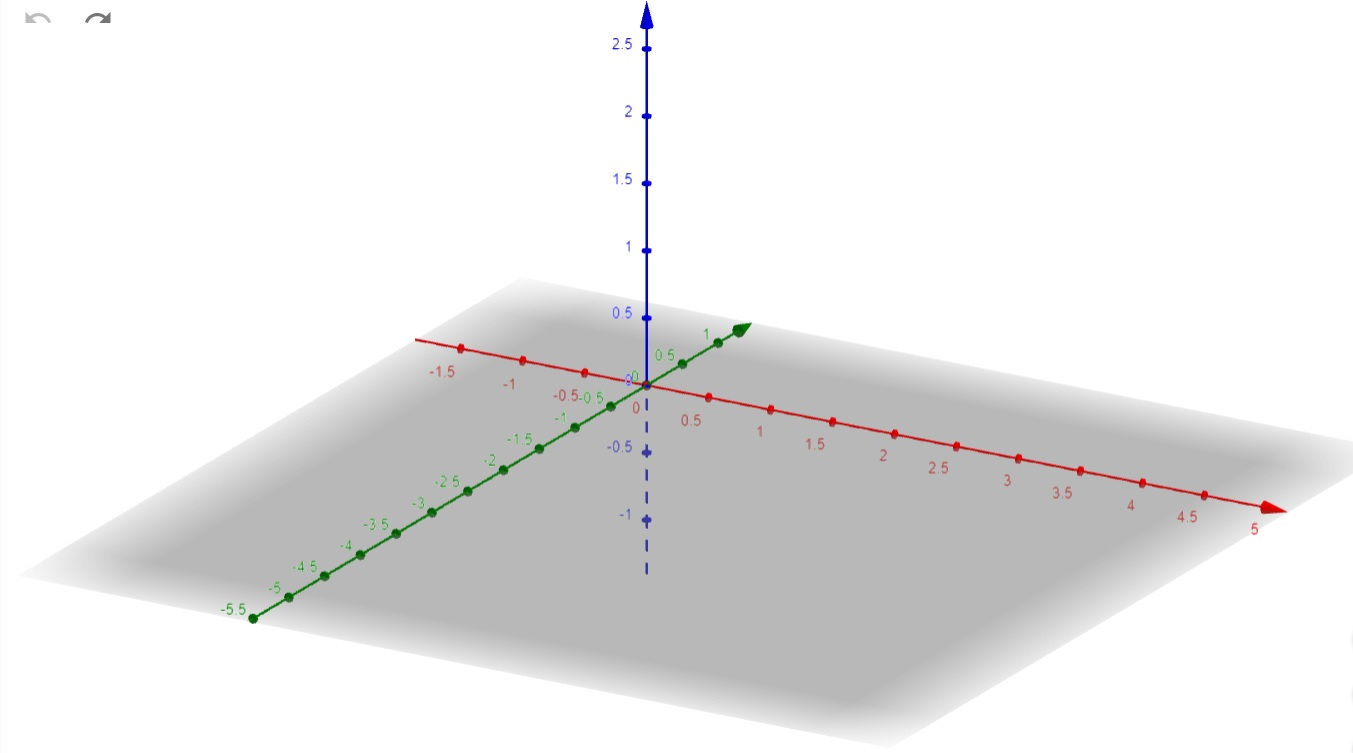
\includegraphics[width=10cm]{graficoquestao3.jpg}
\caption{Representação gráfica.}
\label{fig:graficoquesto3.jpg}
\end{figure}


\begin{itemize}

\item Invente seu subespaço vetorial em qualquer R n com n maior igual a 2. Mostre que o conjunto apresentado é de fato
um subespaço vetorial. Não vale usar nenhum exemplo da aula ou da prova
\end{itemize}

W = \{(x, y, z) \mid  x + y -2z = 0 \} 

 

x + y -2z = 0

x = -y + 2z 

 
W= {(-y + 2z, y, z) \mid y,z \in R\}\\


 

I) (0,0,0) \in W, pois: y,z = 0 \\




II) v, w, x \in W \to  v + w + x \in W, sendo:  

v = (-y1 + 2z1, y1, z1)

w = (-y2 + 2z2, y2, z2)

z = (-y3 + 2z3, y3, z3)

v + w + z  = (-y1 + 2z, y1, -2y1) + (-y2 + 2z2, y2, z2) + (-y3 + 2z3, y3, z3)

u + w + z = (-y1+2z1-y2+2z2-y3+2z3,y1+y2+y3,-2y1+z2+z3) 

Logo, u + w + z \in W\\

III) a \in R, v \in Z \to av \in W. Sendo:  

v = (v1,v2,v3)  \to (-y1 + 2z1, y1, z1)  

a.v = a . (-y1 + 2z1, y1, z1) 

a.v = (a . (-y1 +2z1), a . y1, a . z1) 

a.v = (-ay1 + a2z1, ay1, -az1) 

Logo, av \in W \\

Logo W é subespaço vetorial de R3 \\
\newpage
\section{Exercício 4}\label{ex4}
Mostre que o conjunto \{(−1, 1, 1, 1, 0, 1, 1),(1, 0, −1, 1, 1, −1, 0),(2, 2, 1, 1, −1, 1, 1),
(1, 0, 0, 1, 2, 1, 1),(2, 0, 2, 0, 2, 0, 2),(1, −1, −1, −1, −1, −1, 1),(3, 0, 2, 0, 2, −1, 2)\} forma uma base para o R−espaço vetorial R7. Escreva o vetor (0, 1, 1, 1, 1, 0, 1) nesta base.
\end{itemize}
\\
\textbf{}\\
\\\\\\\\\\
\xrightarrow{Início}
\begin{hbox}{

$\left[
\begin{tabular}{ccccccc|c}
-1 & 1 & 2 & 1 & 2 & 1 & 3 & a\\
1 & 0 & 2 & 0 & 0 & -1 & 0 & b\\
1 & -1 & 1 & 0 & 2 & -1 & 2 & c\\
1 & 1 & 1 & 1 & 0 & -1 & 0 & d\\
0 & 1 & -1 & 2 & 2 & -1 & 2 & e\\
1 & -1 & 1 & 1 & 0 & -1 & -1 & f\\
1 & 0 & 1 & 1 & 2 & 1 & 2 & g\\
\end{tabular}
\right]}
\end{hbox}
\\\\\\\\\\
\begin{hbox}{ 
$
$$\xrightarrow{l2\rightarrow l2+l1}
\\\\
$\left[
\begin{tabular}{ccccccc|c}
-1 & 1 & 2 & 1 & 2 & 1 & 3 & a\\
0 & 1 & 4 & 1 & 2 & 0 & 3 & b+a\\
1 & -1 & 1 & 0 & 2 & -1 & 2 & c\\
1 & 1 & 1 & 1 & 0 & -1 & 0 & d\\
0 & 1 & -1 & 2 & 2 & -1 & 2 & e\\
1 & -1 & 1 & 1 & 0 & -1 & -1 & f\\
1 & 0 & 1 & 1 & 2 & 1 & 2 & g\\
\end{tabular}
\right]\\
$}
\end{hbox}\\
\\\\\\\\\\
\xrightarrow{l3\rightarrow l3+l1}
\begin{hbox}{

$\left[
\begin{tabular}{ccccccc|c}
-1 & 1 & 2 & 1 & 2 & 1 & 3 & a\\
0 & 1 & 4 & 1 & 2 & 0 & 3 & b+a\\
0 & 0 & 3 & 1 & 4 & 0 & 5 & c+a\\
1 & 1 & 1 & 1 & 0 & -1 & 0 & d\\
0 & 1 & -1 & 2 & 2 & -1 & 2 & e\\
1 & -1 & 1 & 1 & 0 & -1 & -1 & f\\
1 & 0 & 1 & 1 & 2 & 1 & 2 & g\\
\end{tabular}
\right]
$}
\end{hbox}

$
\\\\
$$ \xrightarrow{l4\rightarrow l4 + l1}
$\left[
\begin{tabular}{ccccccc|c}
-1 & 1 & 2 & 1 & 2 & 1 & 3 & a\\
0 & 1 & 4 & 1 & 2 & 0 & 3 & b+a\\
0 & 0 & 3 & 1 & 4 & 0 & 5 & c+a\\
0 & 2 & 3 & 2 & 2 & 0 & 3 & d+a\\
0 & 1 & -1 & 2 & 2 & -1 & 2 & e\\
1 & -1 & 1 & 1 & 0 & -1 & -1 & f\\
1 & 0 & 1 & 1 & 2 & 1 & 2 & g\\
\end{tabular}
\right]\\
$
\end{hbox}\\
\\\\\\\\\\
\xrightarrow{l6\rightarrow l6+l1}
\begin{hbox}{

$\left[
\begin{tabular}{ccccccc|c}
-1 & 1 & 2 & 1 & 2 & 1 & 3 & a\\
0 & 1 & 4 & 1 & 2 & 0 & 3 & b+a\\
0 & 0 & 3 & 1 & 4 & 0 & 5 & c+a\\
0 & 2 & 3 & 2 & 2 & 0 & 3 & d+a\\
0 & 1 & -1 & 2 & 2 & -1 & 2 & e\\
0 & 0 & 3 & 2 & 2 & 0 & 2 & f+a\\
1 & 0 & 1 & 1 & 2 & 1 & 2 & g\\
\end{tabular}
\right]

$
$$\xrightarrow{l7\rightarrow l7 + l1}
\\\\
$\left[
\begin{tabular}{ccccccc|c}
-1 & 1 & 2 & 1 & 2 & 1 & 3 & a\\
0 & 1 & 4 & 1 & 2 & 0 & 3 & b+a\\
0 & 0 & 3 & 1 & 4 & 0 & 5 & c+a\\
0 & 2 & 3 & 2 & 2 & 0 & 3 & d+a\\
0 & 1 & -1 & 2 & 2 & -1 & 2 & e\\
0 & 0 & 3 & 2 & 2 & 0 & 2 & f+a\\
0 & 1 & 3 & 2 & 4 & 2 & 5 & g+a\\
\end{tabular}
\right]\\
$
\end{hbox}\\
\\\\\\\\\\
\xrightarrow{l1\rightarrow l1-l2}
\begin{hbox}{

$\left[
\begin{tabular}{ccccccc|c}
-1 & 0 & -2 & 0 & 0 & 1 & 0 & 2a+b\\
0 & 1 & 4 & 1 & 2 & 0 & 3 & b+a\\
0 & 0 & 3 & 1 & 4 & 0 & 5 & c+a\\
0 & 2 & 3 & 2 & 2 & 0 & 3 & d+a\\
0 & 1 & -1 & 2 & 2 & -1 & 2 & e\\
0 & 0 & 3 & 2 & 2 & 0 & 2 & f+a\\
0 & 1 & 3 & 2 & 4 & 2 & 5 & g+a\\
\end{tabular}
\right]

$
$$\xrightarrow{l4\rightarrow l4/2}
\\\\
$\left[
\begin{tabular}{ccccccc|c}
-1 & 0 & -2 & 0 & 0 & 1 & 0 & 2a+b\\
0 & 1 & 4 & 1 & 2 & 0 & 3 & b+a\\
0 & 0 & 3 & 1 & 4 & 0 & 5 & c+a\\
0 & 1 & 3/2 & 0 & 0 & 0 & 3/2 & d+a/2\\
0 & 1 & -1 & 2 & 2 & -1 & 2 & e\\
0 & 0 & 3 & 2 & 2 & 0 & 2 & f+a\\
0 & 1 & 3 & 2 & 4 & 2 & 5 & g+a\\
\end{tabular}
\right]\\
$
\end{hbox}\\
\\\\\\\\\\
\xrightarrow{l4\rightarrow l4-l2}
\begin{hbox}{

$\left[
\begin{tabular}{ccccccc|c}
-1 & 0 & -2 & 0 & 0 & 1 & 0 & 2a+b\\
0 & 1 & 4 & 1 & 2 & 0 & 3 & b+a\\
0 & 0 & 3 & 1 & 4 & 0 & 5 & c+a\\
0 & 0 & -5/2 & 0 & -1 & 0 & -3/2 & d+3a-2b/2\\
0 & 1 & -1 & 2 & 2 & -1 & 2 & e\\
0 & 0 & 3 & 2 & 2 & 0 & 2 & f+a\\
0 & 1 & 3 & 2 & 4 & 2 & 5 & g+a\\
\end{tabular}
\right]

$
$$\xrightarrow{l5\rightarrow l5-l2}
\\\\
$\left[
\begin{tabular}{ccccccc|c}
-1 & 0 & -2 & 0 & 0 & 1 & 0 & 2a+b\\
0 & 1 & 4 & 1 & 2 & 0 & 3 & b+a\\
0 & 0 & 3 & 1 & 4 & 0 & 5 & c+a\\
0 & 0 & -5/2 & 0 & -1 & 0 & -3/2 & d+3a-2b/2\\
0 & 0 & -5 & 1 & 0 & -1 & -1 & e-b+a\\
0 & 0 & 3 & 2 & 2 & 0 & 2 & f+a\\
0 & 1 & 3 & 2 & 4 & 2 & 5 & g+a\\
\end{tabular}
\right]\\
$
\end{hbox}\\
\\\\\\\\\\
\xrightarrow{l7\rightarrow l7-l2}
\begin{hbox}{

$\left[
\begin{tabular}{ccccccc|c}
-1 & 0 & -2 & 0 & 0 & 1 & 0 & 2a+b\\
0 & 1 & 4 & 1 & 2 & 0 & 3 & b+a\\
0 & 0 & 3 & 1 & 4 & 0 & 5 & c+a\\
0 & 0 & -5/2 & 0 & -1 & 0 & -3/2 & d+3a-2b/2\\
0 & 0 & -5 & 1 & 0 & -1 & -1 & e-b+a\\
0 & 0 & 3 & 2 & 2 & 0 & 2 & f+a\\
0 & 0 & -1 & 1 & 2 & 2 & 2 & g+2a-b\\
\end{tabular}
\right]

$
$$\xrightarrow{l3\rightarrow l3/3}
\\\\
$\left[
\begin{tabular}{ccccccc|c}
-1 & 0 & -2 & 0 & 0 & 1 & 0 & 2a+b\\
0 & 1 & 4 & 1 & 2 & 0 & 3 & b+a\\
0 & 0 & 1 & 1/3 & 4/3 & 0 & 5/3 & c+a/3\\
0 & 0 & -5/2 & 0 & -1 & 0 & -3/2 & d+3a-2b/5\\
0 & 0 & -5 & 1 & 0 & -1 & -1 & e-b+a\\
0 & 0 & 3 & 2 & 2 & 0 & 2 & f+a\\
0 & 0 & -1 & 1 & 2 & 2 & 2 & g+2a-b\\
\end{tabular}
\right]\\
$
\end{hbox}\\
\\\\\\\\\\
\xrightarrow{l4\rightarrow -2.5.l4}
\begin{hbox}{

$\left[
\begin{tabular}{ccccccc|c}
-1 & 0 & -2 & 0 & 0 & 1 & 0 & 2a+b\\
0 & 1 & 4 & 1 & 2 & 0 & 3 & b+a\\
0 & 0 & 1 & 1/3 & 4/3 & 0 & 5/3 & c+a/3\\
0 & 0 & 1 & 0 & 2/5 & 0 & 3/5 & -d+3a-2b/5\\
0 & 0 & -5 & 1 & 0 & -1 & -1 & e-b+a/5\\
0 & 0 & 3 & 2 & 2 & 0 & 2 & f+a\\
0 & 0 & -1 & 1 & 2 & 2 & 2 & g+2a-b\\
\end{tabular}
\right]

$
$$\xrightarrow{l5\rightarrow l5/5}
\\\\
$\left[
\begin{tabular}{ccccccc|c}
-1 & 0 & -2 & 0 & 0 & 1 & 0 & 2a+b\\
0 & 1 & 4 & 1 & 2 & 0 & 3 & b+a\\
0 & 0 & 1 & 1/3 & 4/3 & 0 & 5/3 & c+a/3\\
0 & 0 & 1 & 0 & 2/5 & 0 & 3/5 & -d+3a-2b/5\\
0 & 0 & -1 & 1/5 & 0 & -1/5 & -1/5 & e-b+a/5\\
0 & 0 & 3 & 2 & 2 & 0 & 2 & b+a/3\\
0 & 0 & -1 & 1 & 2 & 2 & 2 & g+2a-b\\
\end{tabular}
\right]\\
$
\end{hbox}\\
\\\\\\\\\\
\xrightarrow{l6\rightarrow l6/3}
\begin{hbox}{

$\left[
\begin{tabular}{ccccccc|c}
-1 & 0 & -2 & 0 & 0 & 1 & 0 & 2a+b\\
0 & 1 & 4 & 1 & 2 & 0 & 3 & b+a\\
0 & 0 & 1 & 1/3 & 4/3 & 0 & 5/3 & c+a/3\\
0 & 0 & 1 & 0 & 2/5 & 0 & 3/5 & \(\frac{-3d-14a+6b-2c}{15}\)\\
0 & 0 & -1 & 1/5 & 0 & -1/5 & -1/5 & e-b+a/5\\
0 & 0 & 1 & 2/3 & 2/3 & 0 & 2/3 & f+a/3\\
0 & 0 & -1 & 1 & 2 & 2 & 2 & g+2a-b\\
\end{tabular}
\right]

$
$$\xrightarrow{l4\rightarrow l4-l3}
\\\\
$\left[
\begin{tabular}{ccccccc|c}
-1 & 0 & -2 & 0 & 0 & 1 & 0 & 2a+b\\
0 & 1 & 4 & 1 & 2 & 0 & 3 & b+a\\
0 & 0 & 1 & 1/3 & 4/3 & 0 & 5/3 & c+a/3\\
0 & 0 & 0 & -1/3 & -14/15 & 0 & 16/15 & -3d-14a+6b-3c \\
0 & 0 & -1 & 1/5 & 0 & -1/5 & -1/5 & e-b+a/5\\
0 & 0 & 1 & 2/3 & 2/3 & 0 & 2/3 & f+a/3\\
0 & 0 & -1 & 1 & 2 & 2 & 2 & g+2a-b\\
\end{tabular}
\right]\\
$
\end{hbox}\\
\\\\\\\\\\
\xrightarrow{l5\rightarrow l5+l3}
\begin{hbox}{

$\left[
\begin{tabular}{ccccccc|c}
-1 & 0 & -2 & 0 & 0 & 1 & 0 & 2a+b\\
0 & 1 & 4 & 1 & 2 & 0 & 3 & b+a\\
0 & 0 & 1 & 1/3 & 4/3 & 0 & 5/3 & c+a/3\\
0 & 0 & 0 & -1/3 & -14/15 & 0 & 16/15 & \(\frac{-3d-14a+6b-3c}{15}\)\\
0 & 0 & 0 & 8/15 & 4/3 & -1/5 & 22/15 & \(\frac{8a+3e-3b+3c}{15}\)\\
0 & 0 & 1 & 2/3 & 2/3 & 0 & 2/3 & f+a/3\\
0 & 0 & -1 & 1 & 2 & 2 & 2 & g+2a-b\\
\end{tabular}
\right]

$
$$\xrightarrow{l6\rightarrow l6-l3}
\\\\
$\left[
\begin{tabular}{ccccccc|c}
-1 & 0 & -2 & 0 & 0 & 1 & 0 & 2a+b\\
0 & 1 & 4 & 1 & 2 & 0 & 3 & b+a\\
0 & 0 & 1 & 1/3 & 4/3 & 0 & 5/3 & c+a/3\\
0 & 0 & 0 & -1/3 & -14/15 & 0 & 16/15 & \(\frac{-3d-14a+6b-3c}{15}\)\\
0 & 0 & 0 & 8/15 & 4/3 & -1/5 & 22/15 & \(\frac{8a+3e-3b+3c}{15}\)\\
0 & 0 & 0 & 1/3 & -2/3 & 0 & -1 & f-c/3\\
0 & 0 & -1 & 1 & 2 & 2 & 2 & g+2a-b\\
\end{tabular}
\right]\\
$
\end{hbox}\\
\\\\\\\\\\
\xrightarrow{l7\rightarrow l7+l3}
\begin{hbox}{

$\left[
\begin{tabular}{ccccccc|c}
-1 & 0 & -2 & 0 & 0 & 1 & 0 & 2a+b\\
0 & 1 & 4 & 1 & 2 & 0 & 3 & b+a\\
0 & 0 & 1 & 1/3 & 4/3 & 0 & 5/3 & c+a/3\\
0 & 0 & 0 & -1/3 & -14/15 & 0 & 16/15 & \(\frac{-3d-14a+6b-3c}{15}\)\\ \\
0 & 0 & 0 & 8/15 & 4/3 & -1/5 & 22/15 & \(\frac{8a+3e-3b+3c}{15}\)\\
0 & 0 & 0 & 1/3 & -2/3 & 0 & -1 & f-c/3\\
0 & 0 & 0 & 4/3 & 10/3 & 2 & 11/3 & \(\frac{3g+7a-3b+c}{3}\)\\
\end{tabular}
\right]

$
$$\xrightarrow{l4\rightarrow 3.l4}
\\\\
$\left[
\begin{tabular}{ccccccc|c}
-1 & 0 & -2 & 0 & 0 & 1 & 0 & 2a+b\\
0 & 1 & 4 & 1 & 2 & 0 & 3 & b+a\\
0 & 0 & 1 & 1/3 & 4/3 & 0 & 5/3 & c+a/3\\
0 & 0 & 0 & 1 & 14/5 & 0 & 16/5 & \(\frac{-3d-14a+6b-3c}{5}\)\\
0 & 0 & 0 & 8/15 & 4/3 & -1/5 & 22/15 & \(\frac{8a+3e-3b+3c}{15}\)\\
0 & 0 & 0 & 1/3 & -2/3 & 0 & -1 & f-c/3\\
0 & 0 & 0 & 4/3 & 10/3 & 2 & 11/3 & \(\frac{3g+7a-3b+c}{3}\)\\
\end{tabular}
\right]\\
$
\end{hbox}\\
\\\\\\\\\\
\xrightarrow{l5\rightarrow 15/8.l5}
\begin{hbox}{

$\left[
\begin{tabular}{ccccccc|c}
-1 & 0 & -2 & 0 & 0 & 1 & 0 & 2a+b\\
0 & 1 & 4 & 1 & 2 & 0 & 3 & b+a\\
0 & 0 & 1 & 1/3 & 4/3 & 0 & 5/3 & c+a/3\\
0 & 0 & 0 & 1 & 14/5 & 0 & 16/5 & \(\frac{-3d-14a+6b-3c}{5}\)\\
0 & 0 & 0 & 1 & 5/2 & -3/8 & 11/4 & \(\frac{8a+3e-3b+3c}{8}\)\\
0 & 0 & 0 & 1/3 & -2/3 & 0 & -1 & f-c/3\\
0 & 0 & 0 & 4/3 & 10/3 & 2 & 11/3 & \(\frac{3g+7a-3b+c}{3}\)\\
\end{tabular}
\right]

$
$$\xrightarrow{l6\rightarrow 3.l6}
\\\\
$\left[
\begin{tabular}{ccccccc|c}
-1 & 0 & -2 & 0 & 0 & 1 & 0 & 2a+b\\
0 & 1 & 4 & 1 & 2 & 0 & 3 & b+a\\
0 & 0 & 1 & 1/3 & 4/3 & 0 & 5/3 & c+a/3\\
0 & 0 & 0 & 1 & 14/5 & 0 & 16/5 & \(\frac{-3d-14a+6b-}{5}\)\\
0 & 0 & 0 & 1 & 5/2 & -3/8 & 11/4 & \(\frac{8a+3e-3b+3c}{8}\) \\
0 & 0 & 0 & 1 & -2 & 0 & -3 & f-c\\
0 & 0 & 0 & 4/3 & 10/3 & 2 & 11/3 & \(\frac{3g+7a-3b+c}{3}\) \\
\end{tabular}
\right]\\
$
\end{hbox}\\
\\\\\\\\\\
\xrightarrow{l5\rightarrow l5-l4}
\begin{hbox}{

$\left[
\begin{tabular}{ccccccc|c}
-1 & 0 & -2 & 0 & 0 & 1 & 0 & 2a+b\\
0 & 1 & 4 & 1 & 2 & 0 & 3 & b+a\\
0 & 0 & 1 & 1/3 & 4/3 & 0 & 5/3 & c+a/3\\
0 & 0 & 0 & 1 & 14/5 & 0 & 16/5 & \(\frac{-3d-14a+6b-}{5}\)\\
0 & 0 & 0 & 0 & -3/10 & -3/8 & -9/20 & \(\frac{8a+3e-3b+3c}{8}\)\\
0 & 0 & 0 & 1 & -2 & 0 & -3 & f-c\\
0 & 0 & 0 & 1 & 5/2 & 3/2 & 11/4 & \(\frac{3g+7a-3b+c}{4}\)\\
\end{tabular}
\right]

$
$$\xrightarrow{l6\rightarrow l6-l4}
\\\\
$\left[
\begin{tabular}{ccccccc|c}
-1 & 0 & -2 & 0 & 0 & 1 & 0 & 2a+b\\
0 & 1 & 4 & 1 & 2 & 0 & 3 & b+a\\
0 & 0 & 1 & 1/3 & 4/3 & 0 & 5/3 & c+a/3\\
0 & 0 & 0 & 1 & 14/5 & 0 & 16/5 & \(\frac{-3d-14a+6b-}{5}\)\\
0 & 0 & 0 & 0 & -3/10 & -3/8 & -9/20 & \(\frac{-72a+13e-+55b+15c-24d}{40}\)\\
0 & 0 & 0 & 0 & -24/5 & 0 & -31/5 & f-c\\
0 & 0 & 0 & 1 & 5/2 & 3/2 & 11/4 & \(\frac{3g+7a-3b+c}{4}\)\\
\end{tabular}
\right]\\
$
\end{hbox}\\
\\\\\\\\\\
\xrightarrow{l7\rightarrow l7-l4}
\begin{hbox}{

$\left[
\begin{tabular}{ccccccc|c}
-1 & 0 & -2 & 0 & 0 & 1 & 0 & 2a+b\\\\
0 & 1 & 4 & 1 & 2 & 0 & 3 & b+a\\\\
0 & 0 & 1 & 1/3 & 4/3 & 0 & 5/3 & \(\frac{c+a}{3}\)\\\\\
0 & 0 & 0 & 1 & 14/5 & 0 & 16/5 & - \(\frac{-3d-14a+6b-5c}{5}\)\\\\
0 & 0 & 0 & 0 & -3/10 & -3/8 & -9/20 & \(\frac{-72a+15e+33b-15c-24d}{40}\)\\\\
0 & 0 & 0 & 0 & -24/5 & 0 & -31/5 & \(\frac{5f-10c-3d-14a+6b}{5}\)\\\\
0 & 0 & 0 & 0 & -3/10 & 3/2 & -9/20 & \(\frac{15g-21a+9b-15c-12d}{20}\)\\\\
\end{tabular}
\right]

$
$$\xrightarrow{l5\rightarrow -10/3.l4}
\\\\
$\left[
\begin{tabular}{ccccccc|c}
-1 & 0 & -2 & 0 & 0 & 1 & 0 & 2a+b\\\\
0 & 1 & 4 & 1 & 2 & 0 & 3 & b+a\\\\
0 & 0 & 1 & 1/3 & 4/3 & 0 & 5/3 & \(\frac{c+a}{3}\)\\\\\
0 & 0 & 0 & 1 & 14/5 & 0 & 16/5 & - \(\frac{-3d-14a+6b-5c}{5}\)\\\\
0 & 0 & 0 & 0 & 1 & 5/4 & 3/2 & - \(\frac{-24a+5e+11b-5c-8d}{4}\)\\\\
0 & 0 & 0 & 0 & -24/5 & 0 & -31/5 & \(\frac{5f-10c-3d-14a+6b}{5}\)\\\\
0 & 0 & 0 & 0 & -3/10 & 3/2 & -9/20 & \(\frac{15g-21a+9b-15c-12d}{20}\)\\\\
\end{tabular}
\right]\\
$
\end{hbox}\\
\\\\\\\\\\
\xrightarrow{l6\rightarrow -5/24.l6}
\begin{hbox}{

$\left[
\begin{tabular}{ccccccc|c}
-1 & 0 & -2 & 0 & 0 & 1 & 0 & 2a+b\\\\
0 & 1 & 4 & 1 & 2 & 0 & 3 & b+a\\\\
0 & 0 & 1 & 1/3 & 4/3 & 0 & 5/3 & \(\frac{c+a}{3}\)\\\\\
0 & 0 & 0 & 1 & 14/5 & 0 & 16/5 & - \(\frac{-3d-14a+6b-5c}{5}\)\\\\
0 & 0 & 0 & 0 & 1 & 5/4 & 3/2 & - \(\frac{-24a+5e+11b-5c-8d}{4}\)\\\\
0 & 0 & 0 & 0 & 1 & 0 & 31/24 & - \(\frac{5f-10c-3d-14a+6b}{24}\)\\\\
0 & 0 & 0 & 0 & -3/10 & 3/2 & -9/20 & \(\frac{15g-21a+9b-15c-12d}{20}\)\\\\
\end{tabular}
\right]

$
$$\xrightarrow{l7\rightarrow -10/3.l7}
\\\\
$\left[
\begin{tabular}{ccccccc|c}
-1 & 0 & -2 & 0 & 0 & 1 & 0 & 2a+b\\\\
0 & 1 & 4 & 1 & 2 & 0 & 3 & b+a\\\\
0 & 0 & 1 & 1/3 & 4/3 & 0 & 5/3 & \(\frac{c+a}{3}\)\\\\\
0 & 0 & 0 & 1 & 14/5 & 0 & 16/5 & - \(\frac{-3d-14a+6b-5c}{5}\)\\\\
0 & 0 & 0 & 0 & 1 & 5/4 & 3/2 & - \(\frac{-24a+5e+11b-5c-8d}{4}\)\\\\
0 & 0 & 0 & 0 & 1 & 0 & 31/24 & - \(\frac{5f-10c-3d-14a+6b}{24}\)\\\\
0 & 0 & 0 & 0 & 1 & -5 & 3/2 & - \(\frac{5g+7a+3b-5c-4d}{2}\)\\\\
\end{tabular}
\right]\\
$
\end{hbox}\\
\\\\\\\\\\
\xrightarrow{l6\rightarrow l6-l5}
\begin{hbox}{

$\left[
\begin{tabular}{ccccccc|c}
-1 & 0 & -2 & 0 & 0 & 1 & 0 & 2a+b\\\\
0 & 1 & 4 & 1 & 2 & 0 & 3 & b+a\\\\
0 & 0 & 1 & 1/3 & 4/3 & 0 & 5/3 & \(\frac{c+a}{3}\)\\\\\
0 & 0 & 0 & 1 & 14/5 & 0 & 16/5 & - \(\frac{-3d-14a+6b-5c}{5}\)\\\\
0 & 0 & 0 & 0 & 1 & 5/4 & 3/2 & - \(\frac{-24a+5e+11b-5c-8d}{4}\)\\\\
0 & 0 & 0 & 0 & 0 & -5/4 & -5/24 & \(\frac{-20c+30e-5f-45d-130a+60b}{24}\)\\\\
0 & 0 & 0 & 0 & 1 & -5 & 3/2 & - \(\frac{5g+7a+3b-5c-4d}{2}\)\\\\
\end{tabular}
\right]

$
$$\xrightarrow{l7\rightarrow l7-l5}
\\\\
$\left[
\begin{tabular}{ccccccc|c}
-1 & 0 & -2 & 0 & 0 & 1 & 0 & 2a+b\\\\
0 & 1 & 4 & 1 & 2 & 0 & 3 & b+a\\\\
0 & 0 & 1 & 1/3 & 4/3 & 0 & 5/3 & \(\frac{c+a}{3}\)\\\\\
0 & 0 & 0 & 1 & 14/5 & 0 & 16/5 & - \(\frac{-3d-14a+6b-5c}{5}\)\\\\
0 & 0 & 0 & 0 & 1 & 5/4 & 3/2 & - \(\frac{-24a+5e+11b-5c-8d}{4}\)\\\\
0 & 0 & 0 & 0 & 0 & -5/4 & -5/24 & \(\frac{-20c+30e-5f-45d-130a+60b}{24}\)\\\\
0 & 0 & 0 & 0 & 0 & -25/4 & 0 & \(\frac{-38a+5e-10g+5b+5c}{4}\)\\\\
\end{tabular}
\right]\\
$
\end{hbox}\\
\\\\\\\\\\
\xrightarrow{l6\rightarrow -4/5.l6}
\begin{hbox}{

$\left[
\begin{tabular}{ccccccc|c}
-1 & 0 & -2 & 0 & 0 & 1 & 0 & 2a+b\\\\
0 & 1 & 4 & 1 & 2 & 0 & 3 & b+a\\\\
0 & 0 & 1 & 1/3 & 4/3 & 0 & 5/3 & \(\frac{c+a}{3}\)\\\\\
0 & 0 & 0 & 1 & 14/5 & 0 & 16/5 & - \(\frac{-3d-14a+6b-5c}{5}\)\\\\
0 & 0 & 0 & 0 & 1 & 5/4 & 3/2 & - \(\frac{-24a+5e+11b-5c-8d}{4}\)\\\\
0 & 0 & 0 & 0 & 0 & 1 & 1/6 & - \(\frac{-4c+6e-f-9d-26a+12b}{6}\)\\\\
0 & 0 & 0 & 0 & 0 & -25/4 & 0 & \(\frac{-38a+5e-10g+5b+5c}{4}\)\\\\
\end{tabular}
\right]

$
$$\xrightarrow{l7\rightarrow -4/25.l7}
\\\\
$\left[
\begin{tabular}{ccccccc|c}
-1 & 0 & -2 & 0 & 0 & 1 & 0 & 2a+b\\\\
0 & 1 & 4 & 1 & 2 & 0 & 3 & b+a\\\\
0 & 0 & 1 & 1/3 & 4/3 & 0 & 5/3 & \(\frac{c+a}{3}\)\\\\\
0 & 0 & 0 & 1 & 14/5 & 0 & 16/5 & - \(\frac{-3d-14a+6b-5c}{5}\)\\\\
0 & 0 & 0 & 0 & 1 & 5/4 & 3/2 & - \(\frac{-24a+5e+11b-5c-8d}{4}\)\\\\
0 & 0 & 0 & 0 & 0 & 1 & 1/6 & - \(\frac{-4c+6e-f-9d-26a+12b}{6}\)\\\\
0 & 0 & 0 & 0 & 0 & 1 & 0 & - \(\frac{-38a+5e-10g+5b+5c}{4}\)\\\\
\end{tabular}
\right]\\
$
\end{hbox}\\
\\\\\\\\\\
\xrightarrow{l7\rightarrow l7-l6}
\begin{hbox}{

$\left[
\begin{tabular}{ccccccc|c}
-1 & 0 & -2 & 0 & 0 & 1 & 0 & 2a+b\\\\
0 & 1 & 4 & 1 & 2 & 0 & 3 & b+a\\\\
0 & 0 & 1 & 1/3 & 4/3 & 0 & 5/3 & \(\frac{c+a}{3}\)\\\\\
0 & 0 & 0 & 1 & 14/5 & 0 & 16/5 & - \(\frac{-3d-14a+6b-5c}{5}\)\\\\
0 & 0 & 0 & 0 & 1 & 5/4 & 3/2 & - \(\frac{-24a+5e+11b-5c-8d}{4}\)\\\\
0 & 0 & 0 & 0 & 0 & 1 & 1/6 & - \(\frac{-4c+6e-f-9d-26a+12b}{6}\)\\\\
0 & 0 & 0 & 0 & 0 & 0 & -1/6 & \(\frac{120e-422a+270b-130c-225d+60g-25f}{150}\)\\\\
\end{tabular}
\right]

$
$$\xrightarrow{l7\rightarrow -6.l7}
\\\\
$\left[
\begin{tabular}{ccccccc|c}
-1 & 0 & -2 & 0 & 0 & 1 & 0 & 2a+b\\\\
0 & 1 & 4 & 1 & 2 & 0 & 3 & b+a\\\\
0 & 0 & 1 & 1/3 & 4/3 & 0 & 5/3 & \(\frac{c+a}{3}\)\\\\\
0 & 0 & 0 & 1 & 14/5 & 0 & 16/5 & - \(\frac{-3d-14a+6b-5c}{5}\)\\\\
0 & 0 & 0 & 0 & 1 & 5/4 & 3/2 & - \(\frac{-24a+5e+11b-5c-8d}{4}\)\\\\
0 & 0 & 0 & 0 & 0 & 1 & 1/6 & - \(\frac{-4c+6e-f-9d-26a+12b}{6}\)\\\\
0 & 0 & 0 & 0 & 0 & 0 & 1 & -\(\frac{120e-422a+270b-130c-225d+60g-25f}{25}\)\\\\
\end{tabular}
\right]\\
$
\end{hbox}\\
\\\\\\\\\\
\xrightarrow{l6\rightarrow l6- (1/6.l7)}
\begin{hbox}{

$\left[
\begin{tabular}{ccccccc|c}
-1 & 0 & -2 & 0 & 0 & 1 & 0 & 2a+b\\\\
0 & 1 & 4 & 1 & 2 & 0 & 3 & b+a\\\\
0 & 0 & 1 & 1/3 & 4/3 & 0 & 5/3 & \(\frac{c+a}{3}\)\\\\\
0 & 0 & 0 & 1 & 14/5 & 0 & 16/5 & - \(\frac{-3d-14a+6b-5c}{5}\)\\\\
0 & 0 & 0 & 0 & 1 & 5/4 & 3/2 & \(\frac{-24a+5e+11b-5c-8d}{4}\)\\\\
0 & 0 & 0 & 0 & 0 & 1 & 0 & \(\frac{10g-5e-5c+38a-5b}{25}\)\\\\
0 & 0 & 0 & 0 & 0 & 0 & 1 & -\(\frac{120e-422a+270b-130c-225d+60g-25f}{25}\)\\\\
\end{tabular}
\right]

$
$$\xrightarrow{l5\rightarrow l5-(3/2.l7)}
\\\\
$\left[
\begin{tabular}{ccccccc|c}
-1 & 0 & -2 & 0 & 0 & 1 & 0 & 2a+b\\\\
0 & 1 & 4 & 1 & 2 & 0 & 3 & b+a\\\\
0 & 0 & 1 & 1/3 & 4/3 & 0 & 5/3 & \(\frac{c+a}{3}\)\\\\
0 & 0 & 0 & 1 & 14/5 & 0 & 16/5 & - \(\frac{-3d-14a+6b-5c}{5}\)\\\\
0 & 0 & 0 & 0 & 1 & 5/4 & 0 & \(\frac{595e-1932a+1345b-655c+1150d+360g-150f}{100}\)\\\\
0 & 0 & 0 & 0 & 0 & 1 & 0 &  \(\frac{10g-5e-5c+38a-5b}{25}\)\\\\
0 & 0 & 0 & 0 & 0 & 0 & 1 &  -\(\frac{120e-422a+270b-130c-225d+60g-25f}{25}\)\\\\
\end{tabular}
\right]\\
$
\end{hbox}\\
\\\\\\\\\\

\xrightarrow{l4\rightarrow l4- (16/5.l7)}
\begin{hbox}{

$\left[
\begin{tabular}{ccccccc|c}
-1 & 0 & -2 & 0 & 0 & 1 & 0 & 2a+b\\\\
0 & 1 & 4 & 1 & 2 & 0 & 3 & b+a\\\\
0 & 0 & 1 & 1/3 & 4/3 & 0 & 5/3 & \(\frac{c+a}{3}\)\\\\
0 & 0 & 0 & 1 & 14/5 & 0 & 0 & \(\frac{1920e-3525d-3402a+4170b-1955c+960g-400f}{125}\)\\\\
0 & 0 & 0 & 0 & 1 & 5/4 & 0 & \(\frac{595e-1932a+1345b-655c+1150d+360g-150f}{50}\)\\\\
0 & 0 & 0 & 0 & 0 & 1 & 0 & \(\frac{10g-5e-5c+38a-5b}{25}\)\\\\
0 & 0 & 0 & 0 & 0 & 0 & 1 & -\(\frac{120e-422a+270b-130c-225d+60g-25f}{25}\)\\\\
\end{tabular}
\right]
\\
\\\\\\\\\\


$
$$\xrightarrow{l3\rightarrow l3-(5/3.l7)}

$\left[
\begin{tabular}{ccccccc|c}
-1 & 0 & -2 & 0 & 0 & 1 & 0 & 2a+b\\\\
0 & 1 & 4 & 1 & 2 & 0 & 3 & b+a\\\\
0 & 0 & 1 & 1/3 & 4/3 & 0 & 0 & \(\frac{120e-125c-417a+270b-255d+60g-25f}{15}\)\\\\
0 & 0 & 0 & 1 & 14/5 & 0 & 0 & \(\frac{1920e-3525d-3402a+4170b-1955c+960g-400f}{125}\)\\\\
0 & 0 & 0 & 0 & 1 & 5/4 & 0 & \(\frac{595e-1932a+1345b-655c+1150d+360g-150f}{50}\)\\\\
0 & 0 & 0 & 0 & 0 & 1 & 0 & \(\frac{10g-5e-5c+38a-5b}{25}\)\\\\
0 & 0 & 0 & 0 & 0 & 0 & 1 & -\(\frac{120e-422a+270b-130c-225d+60g-25f}{25}\)\\\\
\end{tabular}
\right]
\end{hbox}\\
\\\\\\\\\\

\xrightarrow{l2\rightarrow l2 - (3.l7)}
\begin{hbox}{

$\left[
\begin{tabular}{ccccccc|c}
-1 & 0 & -2 & 0 & 0 & 1 & 0 & 2a+b\\\\
0 & 1 & 4 & 1 & 2 & 0 & 0 & \(\frac{360e+835b-1214a-390c-675d+180g-75f}{25}\)\\\\
0 & 0 & 1 & 1/3 & 4/3 & 0 & 0 & \(\frac{120e-125c-417a+270b-255d+60g-25f}{15}\)\\\\
0 & 0 & 0 & 1 & 14/5 & 0 & 0 & \(\frac{1920e-3525d-3402a+4170b-1955c+960g-400f}{125}\)\\\\
0 & 0 & 0 & 0 & 1 & 5/4 & 0 & \(\frac{595e-1932a+1345b-655c+1150d+360g-150f}{50}\)\\\\
0 & 0 & 0 & 0 & 0 & 1 & 0 & \(\frac{10g-5e-5c+38a-5b}{25}\)\\\\
0 & 0 & 0 & 0 & 0 & 0 & 1 & -\(\frac{120e-422a+270b-130c-225d+60g-25f}{25}\)\\\\
\end{tabular}
\right]
\\
\\\\\\\\\\


$
$$\xrightarrow{l5\rightarrow l5-(5/4.l6)}

$\left[
\begin{tabular}{ccccccc|c}
-1 & 0 & -2 & 0 & 0 & 1 & 0 & 2a+b\\\\
0 & 1 & 4 & 1 & 2 & 0 & 0 & \(\frac{360e+835b-1214a-390c-675d+180g-75f}{25}\)\\\\
0 & 0 & 1 & 1/3 & 4/3 & 0 & 0 & \(\frac{120e-125c-417a+270b-255d+60g-25f}{15}\)\\\\
0 & 0 & 0 & 1 & 14/5 & 0 & 0 & \(\frac{1920e-3525d-3402a+4170b-1955c+960g-400f}{125}\)\\\\
0 & 0 & 0 & 0 & 1 & 0 & 0 & \(\frac{60e-1061a+685b-315c+575d+155g-75f}{50}\)\\\\
0 & 0 & 0 & 0 & 0 & 1 & 0 & \(\frac{10g-5e-5c+38a-5b}{25}\)\\\\
0 & 0 & 0 & 0 & 0 & 0 & 1 & -\(\frac{120e-422a+270b-130c-225d+60g-25f}{25}\)\\\\
\end{tabular}
\right]
\end{hbox}\\
\\\\\\\\\\

\xrightarrow{l1\rightarrow l1 - l6}
\begin{hbox}{

$\left[
\begin{tabular}{ccccccc|c}
-1 & 0 & -2 & 0 & 0 & 0 & 0 & \(\frac{12a+5e+30b-10g+5c}{25}\)\\\\
0 & 1 & 4 & 1 & 2 & 0 & 0 & \(\frac{360e+835b-1214a-390c-675d+180g-75f}{25}\)\\\\
0 & 0 & 1 & 1/3 & 4/3 & 0 & 0 & \(\frac{120e-125c-417a+270b-255d+60g-25f}{15}\)\\\\
0 & 0 & 0 & 1 & 14/5 & 0 & 0 & \(\frac{1920e-3525d-3402a+4170b-1955c+960g-400f}{125}\)\\\\
0 & 0 & 0 & 0 & 1 & 0 & 0 & \(\frac{60e-1061a+685b-315c+575d+155g-75f}{50}\)\\\\
0 & 0 & 0 & 0 & 0 & 1 & 0 & \(\frac{10g-5e-5c+38a-5b}{25}\)\\\\
0 & 0 & 0 & 0 & 0 & 0 & 1 & -\(\frac{120e-422a+270b-130c-225d+60g-25f}{25}\)\\\\
\end{tabular}
\right]
\\
\\\\\\\\\\


$
$$\xrightarrow{l4\rightarrow l4-(14/5.l5)}

$\left[
\begin{tabular}{ccccccc|c}
-1 & 0 & -2 & 0 & 0 & 0 & 0 & \(\frac{12a+5e+30b-10g+5c}{25}\)\\\\
0 & 1 & 4 & 1 & 2 & 0 & 0 & \(\frac{360e+835b-1214a-390c-675d+180g-75f}{25}\)\\\\
0 & 0 & 1 & 1/3 & 4/3 & 0 & 0 & \(\frac{120e-125c-417a+270b-255d+60g-25f}{15}\)\\\\
0 & 0 & 0 & 1 & 0 & 0 & 0 & \(\frac{16g+60e-302d+161a-25b+10c-16f}{5}\)\\\\
0 & 0 & 0 & 0 & 1 & 0 & 0 & \(\frac{60e-1061a+685b-315c+575d+155g-75f}{50}\)\\\\
0 & 0 & 0 & 0 & 0 & 1 & 0 & \(\frac{10g-5e-5c+38a-5b}{25}\)\\\\
0 & 0 & 0 & 0 & 0 & 0 & 1 & -\(\frac{120e-422a+270b-130c-225d+60g-25f}{25}\)\\\\
\end{tabular}
\right]
\end{hbox}\\
\\\\\\\\\\

\xrightarrow{l3\rightarrow l3 - (4/3.l5)}
\begin{hbox}{

$\left[
\begin{tabular}{ccccccc|c}
-1 & 0 & -2 & 0 & 0 & 0 & 0 & \(\frac{12a+5e+30b-10g+5c}{25}\)\\\\
0 & 1 & 4 & 1 & 2 & 0 & 0 & \(\frac{360e+835b-1214a-390c-675d+180g-75f}{25}\)\\\\
0 & 0 & 1 & 1/3 & 0 & 0 & 0 & \(\frac{260g+620e-605c-2237a+1370b-1275d-125f}{75}\)\\\\
0 & 0 & 0 & 1 & 0 & 0 & 0 & \(\frac{16g+60e-302d+161a-25b+10c-16f}{5}\)\\\\
0 & 0 & 0 & 0 & 1 & 0 & 0 & \(\frac{60e-1061a+685b-315c+575d+155g-75f}{50}\)\\\\
0 & 0 & 0 & 0 & 0 & 1 & 0 & \(\frac{10g-5e-5c+38a-5b}{25}\)\\\\
0 & 0 & 0 & 0 & 0 & 0 & 1 & -\(\frac{120e-422a+270b-130c-225d+60g-25f}{25}\)\\\\
\end{tabular}
\right]
\\
\\\\\\\\\\


$
$$\xrightarrow{l2\rightarrow l2-(2.l5)}

$\left[
\begin{tabular}{ccccccc|c}
-1 & 0 & -2 & 0 & 0 & 0 & 0 & \(\frac{12a+5e+30b-10g+5c}{25}\)\\\\
0 & 1 & 4 & 1 & 0 & 0 & 0 & \(\frac{74e+169b-258a-76c-135d+32g-15f}{5}\)\\\\
0 & 0 & 1 & 1/3 & 0 & 0 & 0 & \(\frac{260g+620e-605c-2237a+1370b-1275d-125f}{75}\)\\\\
0 & 0 & 0 & 1 & 0 & 0 & 0 & \(\frac{16g+60e-302d+161a-25b+10c-16f}{5}\)\\\\
0 & 0 & 0 & 0 & 1 & 0 & 0 & \(\frac{60e-1061a+685b-315c+575d+155g-75f}{50}\)\\\\
0 & 0 & 0 & 0 & 0 & 1 & 0 & \(\frac{10g-5e-5c+38a-5b}{25}\)\\\\
0 & 0 & 0 & 0 & 0 & 0 & 1 & -\(\frac{120e-422a+270b-130c-225d+60g-25f}{25}\)\\\\
\end{tabular}
\right]
\end{hbox}\\
\\\\\\\\\\

\xrightarrow{l3\rightarrow l3 - (1/3.l4)}
\begin{hbox}{

$\left[
\begin{tabular}{ccccccc|c}
-1 & 0 & -2 & 0 & 0 & 0 & 0 & \(\frac{12a+5e+30b-10g+5c}{25}\)\\\\
0 & 1 & 4 & 1 & 0 & 0 & 0 & \(\frac{74e+169b-258a-76c-135d+32g-15f}{5}\)\\\\
0 & 0 & 1 & 0 & 0 & 0 & 0 & \(\frac{180g+320e-655c-3042a+1495b+235d-45f}{75}\)\\\\
0 & 0 & 0 & 1 & 0 & 0 & 0 & \(\frac{16g+60e-302d+161a-25b+10c-16f}{5}\)\\\\
0 & 0 & 0 & 0 & 1 & 0 & 0 & \(\frac{60e-1061a+685b-315c+575d+155g-75f}{50}\)\\\\
0 & 0 & 0 & 0 & 0 & 1 & 0 & \(\frac{10g-5e-5c+38a-5b}{25}\)\\\\
0 & 0 & 0 & 0 & 0 & 0 & 1 & -\(\frac{120e-422a+270b-130c-225d+60g-25f}{25}\)\\\\
\end{tabular}
\right]
\\
\\\\\\\\\\

$
$$\xrightarrow{l2\rightarrow l2-l4}

$\left[
\begin{tabular}{ccccccc|c}
-1 & 0 & -2 & 0 & 0 & 0 & 0 & \(\frac{12a+5e+30b-10g+5c}{25}\)\\\\
0 & 1 & 4 & 0 & 0 & 0 & 0 & \(\frac{16g+14e+194b-419a-86c+167d+f}{5}\)\\\\
0 & 0 & 1 & 0 & 0 & 0 & 0 & \(\frac{180g+320e-655c-3042a+1495b+235d-45f}{75}\)\\\\
0 & 0 & 0 & 1 & 0 & 0 & 0 & \(\frac{16g+60e-302d+161a-25b+10c-16f}{5}\)\\\\
0 & 0 & 0 & 0 & 1 & 0 & 0 & \(\frac{60e-1061a+685b-315c+575d+155g-75f}{50}\)\\\\
0 & 0 & 0 & 0 & 0 & 1 & 0 & \(\frac{10g-5e-5c+38a-5b}{25}\)\\\\
0 & 0 & 0 & 0 & 0 & 0 & 1 & -\(\frac{120e-422a+270b-130c-225d+60g-25f}{25}\)\\\\
\end{tabular}
\right]
\end{hbox}\\
\\\\\\\\\\

\xrightarrow{l2\rightarrow l2 - (4.l3)}
\begin{hbox}{

$\left[
\begin{tabular}{ccccccc|c}
-1 & 0 & -2 & 0 & 0 & 0 & 0 & \(\frac{12a+5e+30b-10g+5c}{25}\)\\\\
0 & 1 & 0 & 0 & 0 & 0 & 0 & \(\frac{-480g-1070e-3070b+5883a+1330c+1565d+195f}{75}\)\\\\
0 & 0 & 1 & 0 & 0 & 0 & 0 & \(\frac{180g+320e-655c-3042a+1495b+235d-45f}{75}\)\\\\
0 & 0 & 0 & 1 & 0 & 0 & 0 & \(\frac{16g+60e-302d+161a-25b+10c-16f}{5}\)\\\\
0 & 0 & 0 & 0 & 1 & 0 & 0 & \(\frac{60e-1061a+685b-315c+575d+155g-75f}{50}\)\\\\
0 & 0 & 0 & 0 & 0 & 1 & 0 & \(\frac{10g-5e-5c+38a-5b}{25}\)\\\\
0 & 0 & 0 & 0 & 0 & 0 & 1 & -\(\frac{120e-422a+270b-130c-225d+60g-25f}{25}\)\\\\
\end{tabular}
\right]
\\
\\\\\\\\\\


$
$$\xrightarrow{l1\rightarrow l1+(2.l3)}

$\left[
\begin{tabular}{ccccccc|c}
-1 & 0 & 0 & 0 & 0 & 0 & 0 & \(\frac{330g+655e-6048a+3080b-1295c+470d-90f}{75}\)\\\\
0 & 1 & 0 & 0 & 0 & 0 & 0 & \(\frac{-480g-1070e-3070b+5883a+1330c+1565d+195f}{75}\)\\\\
0 & 0 & 1 & 0 & 0 & 0 & 0 & \(\frac{180g+320e-655c-3042a+1495b+235d-45f}{75}\)\\\\
0 & 0 & 0 & 1 & 0 & 0 & 0 & \(\frac{16g+60e-302d+161a-25b+10c-16f}{5}\)\\\\
0 & 0 & 0 & 0 & 1 & 0 & 0 & \(\frac{60e-1061a+685b-315c+575d+155g-75f}{50}\)\\\\
0 & 0 & 0 & 0 & 0 & 1 & 0 & \(\frac{10g-5e-5c+38a-5b}{25}\)\\\\
0 & 0 & 0 & 0 & 0 & 0 & 1 & -\(\frac{120e-422a+270b-130c-225d+60g-25f}{25}\)\\\\
\end{tabular}
\right]
\end{hbox}\\
\\\\\\\\\\

$$\xrightarrow{l1\rightarrow -1.l1}
\begin{hbox}{

$\left[
\begin{tabular}{ccccccc|c}
1 & 0 & 0 & 0 & 0 & 0 & 0 & - \(\frac{330g+655e-6048a+3080b-1295c+470d-90f}{75}\)\\\\
0 & 1 & 0 & 0 & 0 & 0 & 0 & \(\frac{-480g-1070e-3070b+5883a+1330c+1565d+195f}{75}\)\\\\
0 & 0 & 1 & 0 & 0 & 0 & 0 & \(\frac{180g+320e-655c-3042a+1495b+235d-45f}{75}\)\\\\
0 & 0 & 0 & 1 & 0 & 0 & 0 & \(\frac{16g+60e-302d+161a-25b+10c-16f}{5}\)\\\\
0 & 0 & 0 & 0 & 1 & 0 & 0 & \(\frac{60e-1061a+685b-315c+575d+155g-75f}{50}\)\\\\
0 & 0 & 0 & 0 & 0 & 1 & 0 & \(\frac{10g-5e-5c+38a-5b}{25}\)\\\\
0 & 0 & 0 & 0 & 0 & 0 & 1 & -\(\frac{120e-422a+270b-130c-225d+60g-25f}{25}\)\\\\
\end{tabular}\\
\right]\\
\end{hbox}\\
\\\\\\\\\\



\section{Coordenadas}\label{ex4}
Portanto o conjunto forma base para o espaço vetorial R7 e as coordenadas são {B = {\(\frac{216}{5}\); -23; 21; \(\frac{-241}{5}\); \(\frac{217}{10}\); 15; \(\frac{19}{5}\)}
\\\\
\end{itemize}
\end{document}
